
\begin{figure}[htbp]
    \begin{minipage}{0.5\hsize}
        \begin{center}
            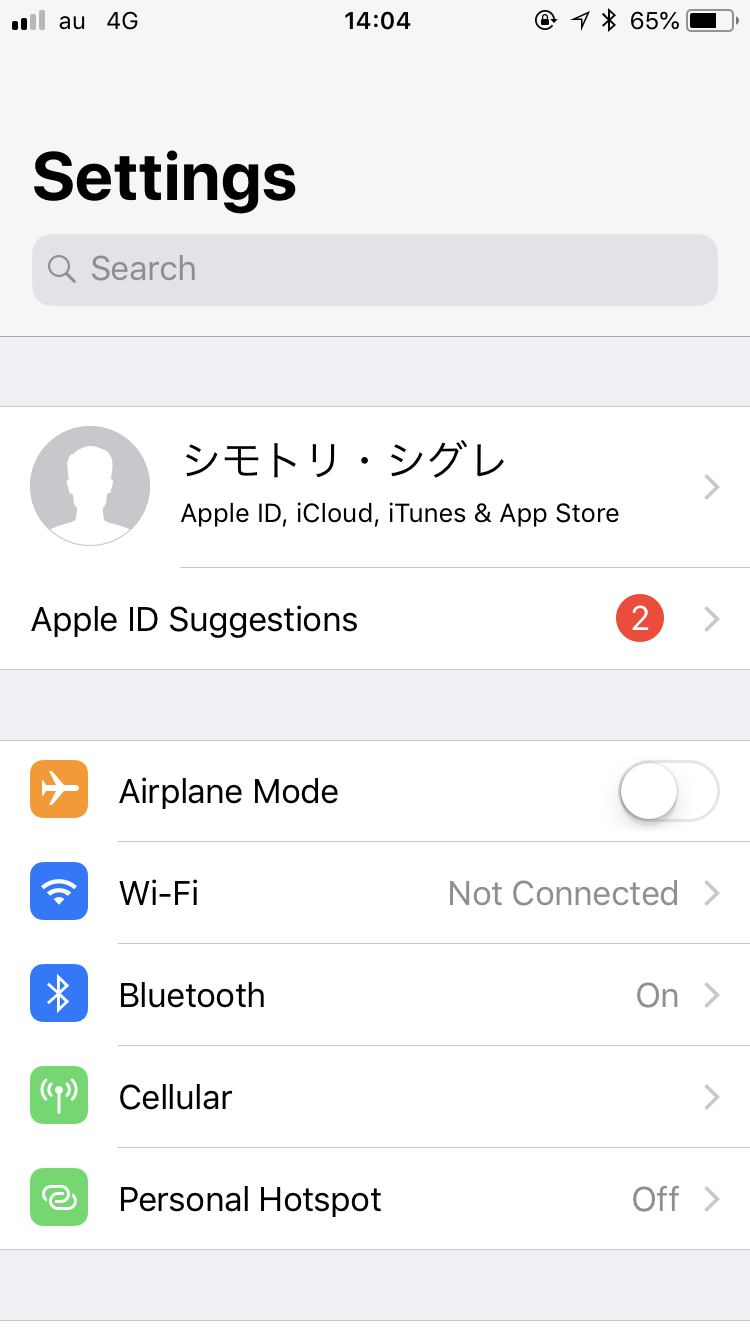
\includegraphics[width=\linewidth]{images/ios_preferences_ltr.png}
        \end{center}
        \caption{英語}
    \end{minipage}
    \begin{minipage}{0.5\hsize}
        \begin{center}
            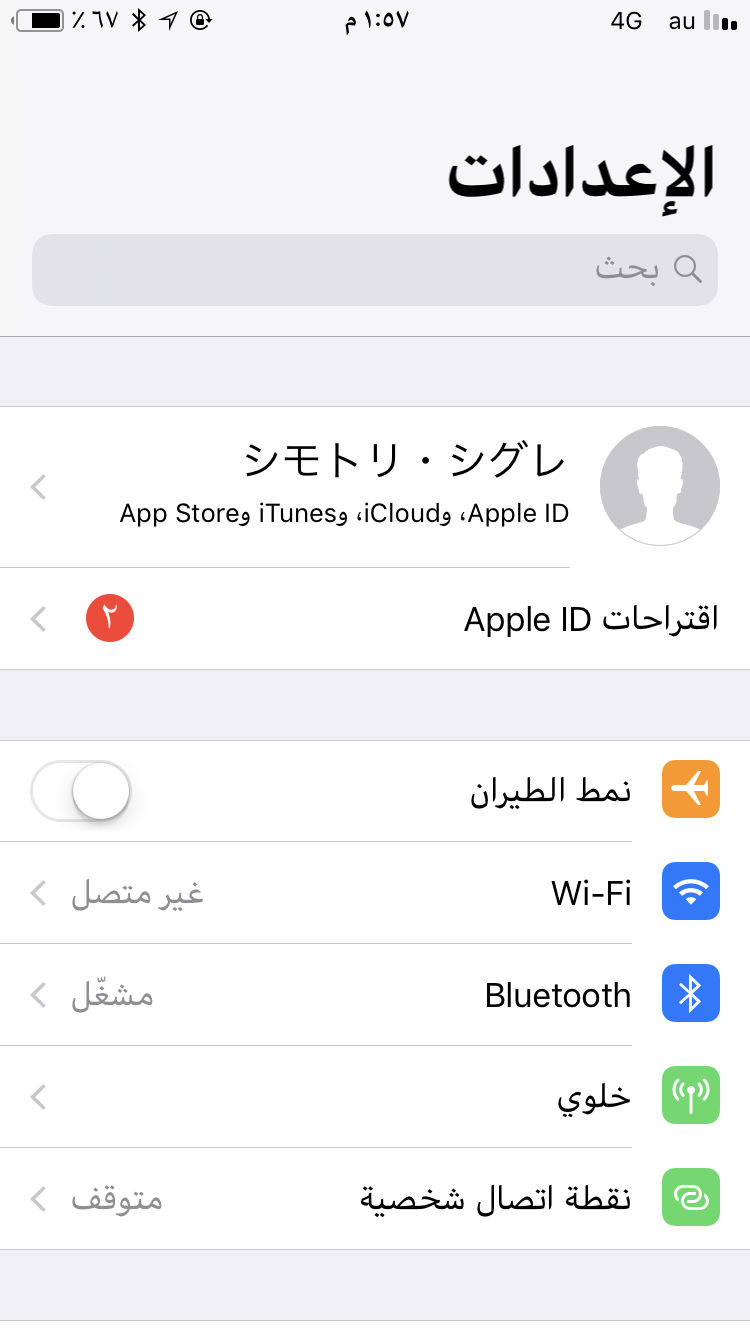
\includegraphics[width=\linewidth]{images/ios_preferences_rtl.png}
        \end{center}
        \caption{アラビア語}
    \end{minipage}
\end{figure}

iOS9からright-to-left言語がサポートされた.Auto Layoutではleading/trailingに対して制約をつけられるようになり,stack viewが新しく使えるようになった\cite{developer.apple.com:videos/play/wwdc2016/232/}\cite{developer.apple.com:library/archive/releasenotes/General/RN-iOSSDK-9.0/index.html}.Auto Layout,stack view,grid viewは自動的に反転される.

base internationalが有効かつAuto Layoutを使用していれば,ある程度はright-to-left言語に合った表示に自動的に切り替わる\footnote{Googleと同じ方針\cite{material.io/design/usability/bidirectionality.html}を取っているように見える.}\cite{developer.apple.com:library/archive/documentation/MacOSX/Conceptual/BPInternational/SupportingRight-To-LeftLanguages/SupportingRight-To-LeftLanguages.html}.

